\documentclass[jair,twoside,11pt,theapa]{article}
\usepackage{jair, theapa, rawfonts}
\usepackage{graphicx}  % include figures
\usepackage{amsmath}  % for centering equations

\jairheading{?}{YYYY}{1-??}{M/YY}{M/YY}
\ShortHeadings{Standard Machine Learning Language (SML)}
{Ikegwu, Hao, \& Brunner}
\firstpageno{1}

\begin{document}

\title{Standard Machine Learning Language}

\author{\name Kelechi Ikegwu \email ikegwu2@illinois.edu \\
       \addr 226 Astronomy Building, MC-??? \\1002 W. Green St.\\ Urbana, IL  61801
       \AND
       \name Micheal Hao  \email ???@illinois.edu \\
       \addr ???
       \AND
       \name Robert Brunner \email bigdog@illinois.edu\\
       \addr 226 Astronomy Building, MC-221 \\1002 W. Green St.\\ Urbana, IL  61801}

% For research notes, remove the comment character in the line below.
% \researchnote

\maketitle


\begin{abstract}
Standard Machine Learning Language (SML) is a language agnostic framework that integrates a query-like language to simplify the development for a variety of state-of-the-art machine learning pipelines. Emphasis was placed on ease of use and abstracting the complexities of machine learning from the end user encouraging it's use in professional and academic settings from a variety of disciplines. SML's architecture is discussed, followed by multiple interfaces that one could use to interact with SML. We then apply SML to a few research problems and compare the complexities for multiple problems. Lastly we perform a case study on SML. The source code and documentation for SML is open sourced and publicly available on github \cite{ginsberg}.
\end{abstract}

\section{Introduction}
\label{Introduction}

Machine Learning has simplified the process of solving a vast amount problems in a variety of fields by learning from data. In most cases machine learning has become more attractive than manually creating programs to solve these same issues. However they're a lot of nuisances (that a novice may be unfamilar with) involved when developing machine learning pipelines \cite{pedros:fewUsefulThings} and if they are not taken into consideration one may not receive satisfactory results. In addition to this, an experience user may not want to deal with [REASONS HERE]. In this paper we introduce Standard Machine Learning Language (SML)  which helps to combat these two use cases.


The overall objective of the SML is to provide a level of abstraction which simplifies the development process of machine learning pipelines. Consequently this enables researchers and industry professionals without a background in this area to use machine learning to solve problems. We developed a query like language to which serves as an abstraction from writing actual machine learning code see Figure \ref{fig:sml-ex-1} for an example.   

\begin{figure}
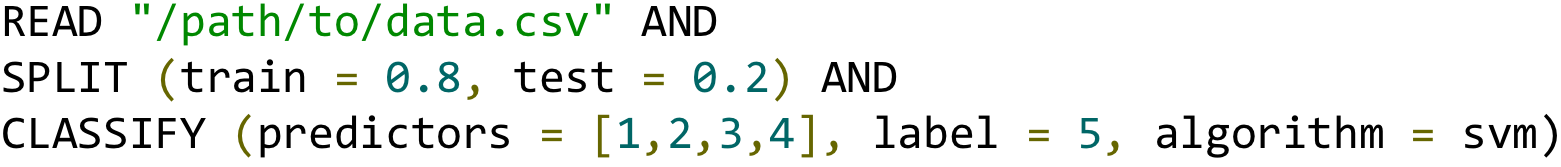
\includegraphics[width=0.6\textwidth]{figs/sml-ex-1.png}
\centering
\caption{Example of a SML Query. TODO: FIX COLOR SYNTAX}
\label{fig:sml-ex-1}
\end{figure}

\section{Related Works}
\label{RelatedWorks}

TPOT \cite{TPOT} is a tool implemented in python that creates and optimizies machine learning pipelines. Given cleaned data, TPOT performs feature selection, preprocessing , and construction. Given the task (classification, regression, or clustering) it uses the best features to determine the most optimal model to use. Lastly, it performs optimization on parameters for the selected model. What differentiates TPOT from SML is that in addition feature, model, and parameter selction/optimization a framework is explictly in place to apply these models to different datasets and construct visualizations for different metrics with each algorithm.

\section{Grammar}
\label{grammar}

The SML language is a domain specific language with grammar implemented in Bakus-Naur form (BNF) \cite{BNF}. Each expression has a rule and can be expanded into other terms. Figure \ref{fig:sml-ex-1} is a typical example of how one would perform classifcation on a dataset. The query in Figure \ref{fig:sml-ex-1} reads in a dataset, peforms a split 80/20 split of training and testing data respectively, and performs classifcation of the 5th column of the hypothetical dataset using columns 1-4 as predictors. 

\subsection{Grammar Structure}
In this subsection we define the grammar of SML in terms of BNF. A query can be defined by a delimited list of actions where the delimiter is an "AND" statement; with BNF syntax this is defined as:
\begin{equation} \label{BNF:Query}
<Query> ::= <Action> | <Action> “AND” <Query>
\end{equation}

An action in (\ref{BNF:Query}) follows one of the following structures defined in (\ref{BNF:Action}) where a keyword is required followed by an argument and/or option list.
\begin{equation} \label{BNF:Action}
\begin{split}
<Action> ::= <Keyword> “<Argument>” \\
| <Keyword> “<Argument>” “(”<Option List>“)” \\
| <Keyword> “(”<Option List>“)”
\end{split}
\end{equation}

A keyword is a predefined term associating an Action with a particular string. An Argument generally is a single string surrounded by quotes that specifies a path to a file. Lastly, an Arugment can have a multitude of options (\ref{BNF:Option}) where an Option consist of an OptionName with either an option value or option value list. An OptionName, and OptionValue consist of a single string, an OptionList (\ref{BNF:OptionList}) consist of a comma delimited list of options and an OptionValueList (\ref{BNF:OptionValueList}) consist of a comma delimited list of OptionValues.

\begin{equation} \label{BNF:Option}
\begin{split}
<Option> ::= <Option Name> “=” <Option Value> \\
		| <Option Name> “=” “[”<Option Value List>“]”
\end{split}
\end{equation}

\begin{equation} \label{BNF:OptionList}
\begin{split}
	<Option List> ::= <Option> | <Option> “,” <Option List>
\end{split}
\end{equation}

\begin{equation} \label{BNF:OptionValueList}
\begin{split}
<Option Value List> ::= <Option Value> \\
| <Option Value> “,” <Option Value List>
\end{split}
\end{equation}

Figure \ref{SML:BNFComp} % figure that shows Figure 1 and it in BNF format side by side.

\subsection{Keywords}
In this subsection we define all of the available keywords that exist in SML. Currently they're 8 keywords in SML.

\subsubsection{Reading Datasets}
When reading data from SML one must use the \(READ\) keyword followed by an Argument containg a path to the dataset. Figure \ref{SML:READ} shows examples of the \(READ\) keyword being used. \(READ\) also accepts an OptionList, for a full list of the optional arguments can visit \ref{}.

\subsubsection{Cleaning Data}
When NaNs, NAs and/or other troublesome values are present in dataset we clean these values in SML by using the \(REPLACE\) keyword. Figure \ref{SML:REPLACE} shows can exajmple of the \(REPLACE\) keyword being used.  

\subsubsection{Patitioning Datasets}
For majority of the situations in Machine Learning it's often useful to split a dataset into training and testing datasets. This can be achieved in SML by using the \(SPLIT\) keyword. Figure \ref{SML:SPLIT} shows an example utlizing the \(SPLIT\) keyword.

\subsubsection{Using Classification Algorithms}
To use a classification algorithm in SML one would use the \(CLASSIFY\) keyword. SML has the following classification algorithms implemented: Support Vector Machines, Naive Bayes, Random Forest, Logistic Regression, and K-Nearest Neighbors. Figure \ref{SML:CLASSIFY} demonstrates how to use the \(CLASSIFY\) keyword in a query.

\subsubsection{Using Clustering Algorithms}
For clustering algorithms can be invoked by using the \(CLUSTER\) keyword. SML currently has K-Means Clustering implemented. Figure \ref{SML:CLUSTER} demonstrates how to use the \(CLUSTER\) keyword in a query.

\subsubsection{Using Regression Algorithms}
Regression algorithms can be invoked by using the \(REGRESS\) keyword. SML currently has the following regression algorithms implemented:Simple Linear Regression, Ridge Regression, Lasso Regression, and Elastic Net Regression. Figure \ref{SML:REGRESS} demonstrates how to use the \(REGRESS\) keyword in a query.

\subsubsection{Saving/Loading Models}
It's possible to save models and reuse them later. To save a model in SML one would use the \(SAVE\) keyword in a query. To load an existing model from SML one would use the \(LOAD\) keyword in a query. Figure \ref{SML:SAVE_LOAD} show how to save and load a model using SML.

\subsubsection{Visualizating Datasets and Metrics of Algorithms}
When using SML it's possible to visualize datasets or metrics of algorithms (such as learning curves, or ROC curves). To do this the \(PLOT\) keyword must be specified in a query. Figure \ref{SML:PLOT} shows can example of how to use the \(PLOT\) keyword in a query.

\section{SML's Architecture}
\label{sml-architecture}

When SML is given a string, it is passed to the parser. The high level implementation of the grammar is then used to parse through the string to determine the actions to perform. The actions are stored in a dictionary and given to one of the following phases of SML: Model Phase, Apply Phase, or Metrics Phase.


The model phase is generally for constructing a model. The keywords that generally invoke the model phase are: \(READ\), \(REPLACE\), \(CLASSIFY\), \(REGRESS\), and \(CLUSTER\). The apply phase is generally for applying a prexisting model  to new data. The keywords that generally invoke the apply phase are: \(LOAD\), and \(APPLY\). It's often useful to visualize the data that one works with and beneifical to see the performance metrics of a machine learning algorithm. By default if you specify the \(PLOT\) keyword in a query, SML will execute the metrics phase. Figure \ref{fig:metric-phase} displays a block diagram of the metric phase of SML. SML performs a dictionary lookup with the average complexity of O(1) to find specific terms that are in the query. For the example in Figure \ref{fig:metric-phase} we specified `PLOT` which instructs SML to create visualizations, with the `READ` keyword SML will create a lattice plot containing kernel density estimates for each feature. Given an algorithm type such as Classification SML generates plots such as ROC Curves and Validation and Learning Curves. For a comprehensive list for the type of plots that SML can generate visit  \cite{}.

\begin{figure}
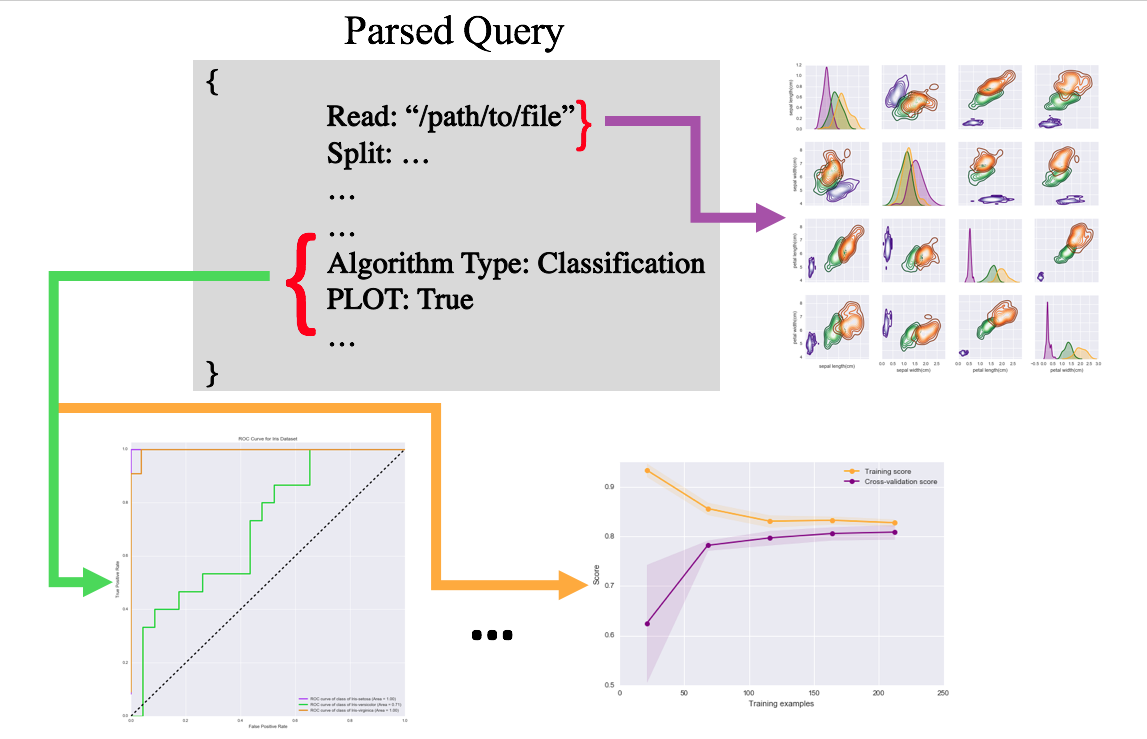
\includegraphics[width=0.6\textwidth]{figs/metric-phase.png}
\centering
\caption{Block Diagram of Metric Phase Architecture}
\label{fig:metric-phase}
\end{figure}

\subsubsection{Connector}
Lastly, another significant component of SML's architecture is the connector. The connector connects Drivers from different languages to achieve an action we want. For instance, consider applying  Linear Regression on a dataset. During the model phase, SML calls the connector to retrieve the linear regression library. SML uses scikit learn's \ref{} implementation for Linear Regression however if we wanted to use a HMM scikit learn removed this algorithm from it's library ergo SML will use the connector to call another library that supports HMM.

\section{Interface}
\label{interface}

They're multiple interfaces available for working with SML. We've developed a web tool that's publicly available which allows the user to interact with SML. There's also a REPL environment available that allows the user to interactively use SML. Lastly, users have the option to import SML into an existing pipeline to simplify the development process.

\section{Use Cases}
\label{use-cases}


We tested the SML framework against ten popular machine learning problems with publicly available data sets. We then selected two problems that researchers have attempted to solve in different domains that utlized machine learning to apply SML. 

\subsection{10 Use Cases}
We applied SML to the following datasets: Iris Dataset \cite{}, Auto-MPG Dataset \cite{}, Seeds Dataset \cite{}, Computer Hardware Dataset \cite{}, Boston Housing Dataset \cite{}, Wine Dataset \cite{}, US Census Dataset \cite{}, Chronic Kidney Disease \cite{}, Spam Detection \cite{}, and the Titanic Dataset \cite{}. In this paper we dicuss applying SML to the Iris Dataset and the Auto-MPG dataset. \cite{Github:DataFlows} provides detailed explanations and examples that solve problems all 10 data sets.

\subsubsection{Iris Dataset}
Figure \ref{SML:IrisQuery} shows all of the code required to perform classification on the Iris dataset. In Figure \ref{SML:IrisQuery} We read data from a specified path, perform a 80/20 split, use the first 4 columns to predict the 5th column, use support vector machines as the algorithm to perform classification and finally plot distributions of our dataset  and metrics of our algorithm. Figure \ref{Manual:IrisCode} illustrates what is required to perform the same operations using scikit learn. The  result for both  snippets of code are the same and can be seen in Figure \ref{IrisResults}.

\subsubsection{Auto-Mpg Dataset}
Figure \ref{SML:AutoMPGQuery} shows all of the code required to perform regression on the Auto-MPG dataset. In Figure \ref{SML:AutoMPGQuery} we read data from a specified path, the dataset is separated by fixed width spaces and we choose not to provide a header for the dataset.  Next we perform a 80/20 split, replace all occurrences of "?" with the mode of the column. We then perform linear regression using columns 2-8 to predict the 1st label. Lastly, we visualize distributions of our dataset and metrics of our algorithm. Figure \ref{Manual:Auto-MPG} demonstrates what's required to perform the same operations using scikit learn. The outcome for both process are the same and can be seen in Figure \ref{AutoMPGResults}

\subsection{Insider Threat Detection}

\subsection{Predicting Health Care Cost Among Medicare beneficiaries in Massachusetts }

\subsection{Discussion}


\section{Future Work}
\label{future-work}

future work stuff

\section{Conclusion}
\label{conclusion}
conclusion stuff

\acks{acknowledgments go here}

\appendix
\section*{Appendix X...}

Appendix goes here if needed.

\vskip 0.2in
\bibliography{main}
\bibliographystyle{theapa}

\end{document}






